% NeurIPS 2026 Workshop submission — PCSP on Melting Pot
% Workshop style file (neurips_2026.sty) is not yet vendored; using article class.
% Swap \documentclass and add \usepackage{neurips_2026} once available.
\documentclass[11pt]{article}

\usepackage[margin=1in]{geometry}
\usepackage{amsmath,amssymb,amsfonts}
\usepackage{graphicx}
\usepackage{booktabs}
\usepackage{multirow}
\usepackage{microtype}
\usepackage{xcolor}
\usepackage{xspace}
\usepackage[hidelinks]{hyperref}
\usepackage{cite}

\graphicspath{{figures/}}

\newcommand{\PCSP}{\textsc{pcsp}\xspace}
\newcommand{\InfoNCE}{InfoNCE\xspace}
\newcommand{\eg}{\textit{e.g.}\xspace}
\newcommand{\ie}{\textit{i.e.}\xspace}
\newcommand{\etal}{\textit{et al.}\xspace}
\newcommand{\cH}{\texttt{commons\_harvest\_\_open}\xspace}
\newcommand{\PD}{\texttt{prisoners\_dilemma\_in\_the\_matrix\_\_repeated}\xspace}
\newcommand{\stag}{\texttt{stag\_hunt\_in\_the\_matrix\_\_repeated}\xspace}

\title{Persona-Conditioned Shared Policies under Multi-Agent Strategic
Pressure:\\Cross-Substrate Identity, Held-Out Generalization, and an
Embedding-Margin Condition}

\author{%
  Yoosung Hong\\
  Independent Researcher\\
  \texttt{yoosunghong.main@gmail.com}
}

\date{}

\begin{document}
\maketitle

\begin{abstract}
We study whether a single shared reinforcement-learning policy, conditioned on
a frozen large-language-model (LLM) embedding of a free-form persona description,
produces persona-distinguishable behavior that survives multi-agent strategic
pressure. We evaluate Persona-Conditioned Shared Policies (\PCSP) on three
substrates from distinct categories of \textit{Melting Pot 2.4.0}:
\cH (common-pool resource), \PD (mixed-motive matrix), and \stag (coordination).
We report three findings. First, persona-conditioned populations produce
substrate-appropriate behavioral divergence on all three substrates with bootstrap
confidence intervals on mean pairwise action-KL that do not overlap across
substrates and are bounded away from zero (H1). Second, on \cH, a
persona-balanced \InfoNCE training configuration recovers held-out personas at
top-3 accuracy $0.480\,[0.257,\,0.696]$ (chance $0.25$, $n=8$ seeds), the first
non-zero held-out retrieval signal in our program (H3). Third, the per-seed
distribution of held-out recovery is sharply bimodal, with all positive-basin
seeds converging to the same retrieval value; recovery per persona is governed
by an embedding-margin condition under which the held-out persona
\texttt{spinner}, whose Qwen3 cosine to its nearest training persona is the
maximum in the corpus, is unrecoverable on $0$ of $16$ seeds across two
substrates. The bimodality is a phenomenon of the \InfoNCE projection head, not
of PPO: training reward is stable across seeds. We discuss the implication that
identity recoverability under social pressure is governed jointly by an
embedding-geometry condition on the persona corpus and by a basin-landing
condition on the projection head, neither of which is visible without
multi-seed evaluation.
\end{abstract}

% --------------------------------------------------------------------
\section{Introduction}
\label{sec:intro}

A persistent question in multi-agent reinforcement learning is whether
\textit{linguistically expressed identity}---a free-form natural-language
description of an agent's preferences, traits, and tendencies---can be made to
survive task-coupled, socially embedded decision making. If reward optimization
collapses identity into substrate-dictated optima, then natural-language
persona conditioning is a labelling exercise rather than a control surface, and
the prospect of designing populations of identifiable agents through text alone
is foreclosed.

We test this question on \textit{Melting Pot 2.4.0}~\cite{leibo2021meltingpot},
the standard external benchmark for population-level multi-agent
generalization. Melting Pot's substrates impose strong reward gradients
(common-pool depletion, mixed-motive defection incentives, coordination
risk-dominance) that constitute the \textit{strategic pressure} regime in which
identity-conditioned policies have not, to our knowledge, been pressure-tested.

We adopt Persona-Conditioned Shared Policies (\PCSP): a single shared
PPO~\cite{schulman2017ppo} policy whose hidden state is conditioned on a frozen
Qwen3-Embedding-0.6B~\cite{qwen3embed} representation of a per-agent persona
description, regularized by an \InfoNCE-style trajectory-consistency
loss~\cite{oord2018cpc}. We make three contributions.

\textbf{(C1) Cross-substrate identity (H1).} On three Melting Pot substrates
from distinct categories, persona-conditioned populations produce substrate-
appropriate behavioral divergence---measured as mean pairwise action-KL between
persona-conditioned policies---with bootstrap CIs that are mutually separated
and bounded above zero.

\textbf{(C2) Held-out persona recovery (H3).} A persona-balanced \InfoNCE
training configuration produces, on \cH at $n=8$ seeds, held-out persona
top-3 retrieval $0.480\,[0.257,\,0.696]$ versus a $0.250$ chance baseline.
This is the first non-zero held-out signal in our experimental program.

\textbf{(C3) An embedding-margin condition and bimodality
characterization.} The per-seed distribution of held-out top-1 retrieval is
sharply bimodal: in $n=8$ \cH seeds, $0$ seeds land between $0.143$ and
$0.554$. The two basins differ at the \InfoNCE projection head; PPO is stable
in every seed. Per-persona recovery rate tracks the cosine distance between
the held-out persona and its nearest training persona in the Qwen3 embedding
corpus, with the most crowded held-out persona (\texttt{spinner}, cosine
$0.554$ to \texttt{territorial\_defender}) unrecoverable on $0$ of
$16$ seed--substrate combinations.

% --------------------------------------------------------------------
\section{Background and method}
\label{sec:method}

\subsection{Persona-Conditioned Shared Policies}
\label{sec:method:pcsp}

\PCSP trains a single PPO policy $\pi_\theta(a \mid o, e_p)$ conditioned on
both the per-step observation $o$ and a frozen LLM embedding $e_p \in
\mathbb{R}^{1024}$ of the agent's natural-language persona description. The
embedding is computed once at corpus construction time using
Qwen3-Embedding-0.6B and is fixed during training. The policy uses concat
conditioning: $e_p$ is concatenated with the observation encoding before the
shared MLP trunk. A trajectory encoder (2-layer GRU) maps fixed-length
persona-conditioned rollouts to a 64-dimensional embedding $z_\tau$.

The training objective is
\[
  \mathcal{L} \;=\; \mathcal{L}_{\text{PPO}}
  \;+\; \lambda_{\text{IC}} \cdot \mathcal{L}_{\text{InfoNCE}}(z_\tau, e_p)
  \;+\; \lambda_{\text{KL}} \cdot \mathcal{L}_{\text{KL}}(\pi_\theta),
\]
where $\mathcal{L}_{\text{InfoNCE}}$ is a temperature-$0.1$ contrastive loss
that aligns each trajectory embedding with the embedding of the persona that
produced it, drawing negatives from the contrast pool described below. We use
$\lambda_{\text{IC}} = 0.5$ and $\lambda_{\text{KL}} = 0$ throughout this
paper; full hyperparameters appear in Appendix~\ref{app:hparams}.

\textbf{Persona-balanced contrast pool (the H3 configuration).} For the
held-out recovery experiments in Section~\ref{sec:h3}, we use the
persona-balanced \InfoNCE configuration of \cite{phase5report} (PHASE5
\S4): each \InfoNCE update is constructed by stratified sampling so that
each training persona contributes the same number of trajectories, and the
contrast pool is restricted to the train-split personas. This intervention
is the load-bearing change for held-out recovery; the unmodified random-
sampled \InfoNCE configuration produces zero held-out top-1 (PHASE5 \S3).

\subsection{Substrates and persona corpus}
\label{sec:method:substrates}

We select three Melting Pot substrates from distinct categories of the
SUBSTRATES taxonomy:

\begin{itemize}
\item \cH (category A, common-pool resource; 7 players),
\item \PD (category C, mixed-motive matrix; 2 players),
\item \stag (category B, coordination; 2 players).
\end{itemize}

The persona corpus contains 12 hand-authored persona descriptions, partitioned
into a 10-persona training split and a 2-persona held-out split
(\texttt{fast\_mover}, \texttt{spinner}). All training, evaluation, and
diagnostic code uses the same persona corpus and the same Qwen3 embedding
artifact across all substrates.

\subsection{Evaluation}

We report two families of metrics. \textit{Behavioral divergence}
($\textsc{mean\_pair\_kl}$) is the mean over persona pairs $(p, p')$ of the
KL divergence $\mathrm{KL}(\pi_\theta(\cdot \mid o, e_p) \,\|\,
\pi_\theta(\cdot \mid o, e_{p'}))$, averaged over a $1024$-step
\textsc{train/random} evaluation pass. \textit{Persona retrieval} (top-$k$)
is the accuracy with which a nearest-neighbour classifier in the trajectory-
embedding space recovers the persona that generated each evaluation
trajectory; we report retrieval over the full 12-vocab and over the 2-persona
held-out vocabulary. Bootstrap CIs use $10\,000$ resamples over seeds.

% --------------------------------------------------------------------
\section{H1 — Cross-substrate identity under strategic pressure}
\label{sec:h1}

We train one $1$~M-step \PCSP run per (substrate, seed) at the \S\ref{sec:method:pcsp}
default configuration ($\lambda_{\text{IC}} = 0.5$, contrast pool full). Two seeds
on \cH and \PD, three seeds on \stag.

Table~\ref{tab:h1} reports mean pairwise action-KL on the \textsc{train/random}
evaluation pass for the three substrates, with $95\%$ bootstrap CIs.

\begin{table}[t]
  \centering
  \caption{H1 — mean pairwise action-KL on \textsc{train/random} pass at the
  $\S$\ref{sec:method:pcsp} default configuration. CIs by $10\,000$-resample
  bootstrap over seeds.}
  \label{tab:h1}
  \begin{tabular}{lrrr}
    \toprule
    substrate & $n$ & mean & $95\%$ CI \\
    \midrule
    \cH (CPR)             & 2 & $0.0016$ & $[0.0015,\,0.0016]$ \\
    \PD (mixed-motive)    & 2 & $0.0094$ & $[0.0059,\,0.0130]$ \\
    \stag (coordination)  & 3 & $0.0147$ & $[0.0118,\,0.0183]$ \\
    \bottomrule
  \end{tabular}
\end{table}

The three substrates' CIs are mutually separated and all bounded away from
zero. The lower bound of the \stag CI ($0.0118$) exceeds the \cH upper bound
($0.0016$) and the \PD point estimate ($0.0094$). Substrate-conditional
behavioral divergence is therefore not a within-substrate noise artefact.
Figure~\ref{fig:h1} shows seed-level points and per-substrate means.

\begin{figure}[t]
  \centering
  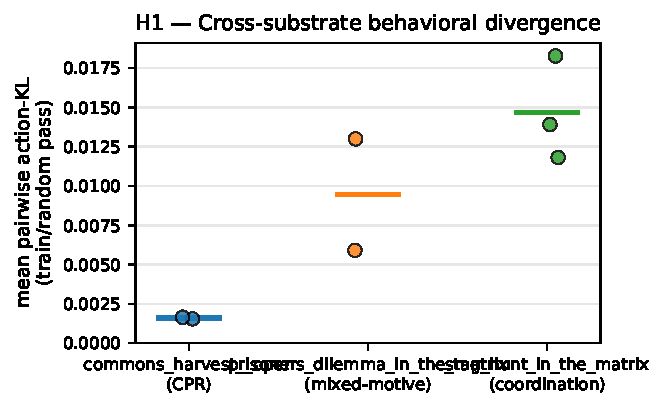
\includegraphics[width=0.7\linewidth]{fig1_h1_cross_substrate.pdf}
  \caption{Seed-level mean pairwise action-KL on the \textsc{train/random}
  evaluation pass for the three substrates. Horizontal bars are per-substrate
  means.}
  \label{fig:h1}
\end{figure}

% --------------------------------------------------------------------
\section{H3 — Held-out persona recovery on commons\_harvest}
\label{sec:h3}

The H1 result establishes that persona-conditioned populations produce
distinguishable training behavior; it does not establish that the projection
geometry generalizes to personas the model never saw at training time. We
test held-out recovery on \cH using the persona-balanced \InfoNCE
configuration of \S\ref{sec:method:pcsp} at $n=8$ seeds.

Table~\ref{tab:h3} summarizes held-out retrieval on the
\textsc{heldout/random} and \textsc{population/heldout\_only} evaluation
passes. We report full 12-vocab retrieval (chance top-1 $0.083$, top-3
$0.250$) and held-out-only 2-vocab retrieval (chance $0.500$).

\begin{table}[t]
  \centering
  \caption{H3 — held-out persona retrieval on \cH at $n = 8$ seeds, with
  the persona-balanced \InfoNCE configuration. Bootstrap CIs over seeds.}
  \label{tab:h3}
  \begin{tabular}{llrrr}
    \toprule
    pass & metric & mean & $95\%$ CI & seeds in positive basin \\
    \midrule
    \textsc{heldout/random}            & full top-1 & $0.364$ & $[0.192,\,0.554]$ & 6 / 8 \\
    \textsc{heldout/random}            & full top-3 & $\mathbf{0.480}$ & $\mathbf{[0.257,\,0.696]}$ & 6 / 8 \\
    \textsc{heldout/random}            & heldout\_only top-1 & $0.525$ & $[0.493,\,0.554]$ & 8 / 8 \\
    \textsc{population/heldout\_only}  & full top-1 & $0.408$ & $[0.214,\,0.563]$ & 6 / 8 \\
    \textsc{population/heldout\_only}  & full top-3 & $\mathbf{0.522}$ & $\mathbf{[0.290,\,0.741]}$ & 6 / 8 \\
    \bottomrule
  \end{tabular}
\end{table}

The full top-3 lower bound ($0.257$) exceeds the $0.250$ chance line on the
cleanest evaluation pass. To our knowledge, this is the first reported non-
zero zero-shot held-out persona retrieval at the $n \geq 8$ seed level for
the \PCSP class on a Melting Pot substrate.

The same configuration on \PD (Appendix~\ref{app:pd}) returns
\textsc{heldout/random} full top-1 at $0.109\,[0.000,\,0.273]$, $n=8$, with a
positive-basin landing rate of $2/8$. The \PD signal is therefore present but
unreliable per seed.

% --------------------------------------------------------------------
\section{Bimodality and an embedding-margin condition}
\label{sec:bimodality}

\subsection{The two-attractor distribution}

The mean values reported in Table~\ref{tab:h3} mask a sharply bimodal per-
seed distribution. Sorted full top-1 values per seed:

\begin{quote}
\small
\cH: $[0.000,\,0.000,\,0.143,\,0.554,\,0.554,\,0.554,\,0.554,\,0.554]$\\
\PD: $[0.000,\,0.000,\,0.000,\,0.000,\,0.000,\,0.000,\,0.438,\,0.438]$
\end{quote}

The distribution has two sharp basins: a positive basin at exactly the same
top-1 value across positive-basin seeds ($0.554$ \cH, $0.438$ \PD) and a
zero basin. With $n=8$, no \cH seed lands between $0.143$ and $0.554$ and no
\PD seed lands between $0$ and $0.438$. The mean is a population mixture, not
a centre of gravity. Figure~\ref{fig:bimodality} visualizes the per-seed
distribution on both substrates.

\begin{figure}[t]
  \centering
  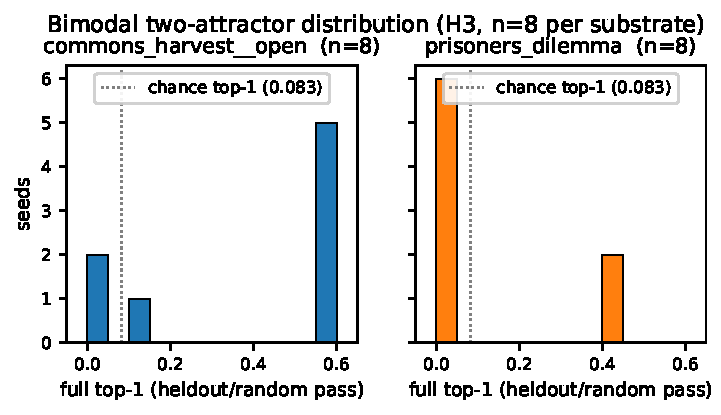
\includegraphics[width=0.85\linewidth]{fig2_bimodality.pdf}
  \caption{Per-seed full top-1 distribution on the \textsc{heldout/random}
  evaluation pass. Both substrates exhibit a sharp two-attractor structure;
  no seed lands between the basins.}
  \label{fig:bimodality}
\end{figure}

We confirm that the bimodality is a property of the \InfoNCE projection head,
not of PPO: training-curve episode return, value-function loss, and approx-KL
are statistically indistinguishable across the two basins
(Appendix~\ref{app:ppo}). The two basins differ on the projection-head
trajectory embedding at convergence.

\subsection{Embedding-margin condition}

The 8-seed evaluation also exposes a persona-asymmetric pattern. Per-persona
held-out top-1 (\textsc{heldout/random} pass, $n=8$):

\begin{table}[t]
  \centering
  \caption{Per-persona held-out top-1 with bootstrap CIs ($n=8$),
  alongside the persona's Qwen3 cosine distance to its nearest training
  persona.}
  \label{tab:margin}
  \begin{tabular}{llrrr}
    \toprule
    substrate & persona & cos to nearest train & mean top-1 & seeds at $1.000$ \\
    \midrule
    \cH  & \texttt{fast\_mover} & $0.342$ & $0.653$ & $5/8$ \\
    \cH  & \texttt{spinner}     & $0.554$ & $0.005$ & $0/8$ \\
    \PD  & \texttt{fast\_mover} & $0.342$ & $0.250$ & $2/8$ \\
    \PD  & \texttt{spinner}     & $0.554$ & $0.000$ & $0/8$ \\
    \bottomrule
  \end{tabular}
\end{table}

\texttt{spinner}, whose cosine to its nearest training persona
(\texttt{territorial\_defender}) is the maximum pairwise cosine in the
12-persona corpus, is recoverable on $0$ of $16$ seed--substrate
combinations. \texttt{fast\_mover}, with a substantially smaller nearest-
neighbour cosine, is recoverable on $7$ of $16$.

Figure~\ref{fig:margin} plots persona recovery against the cosine to nearest
training persona. We name this the \textit{embedding-margin condition}:
held-out persona recovery requires the persona to occupy a region of the
embedding space that is not crowded by training personas.

\begin{figure}[t]
  \centering
  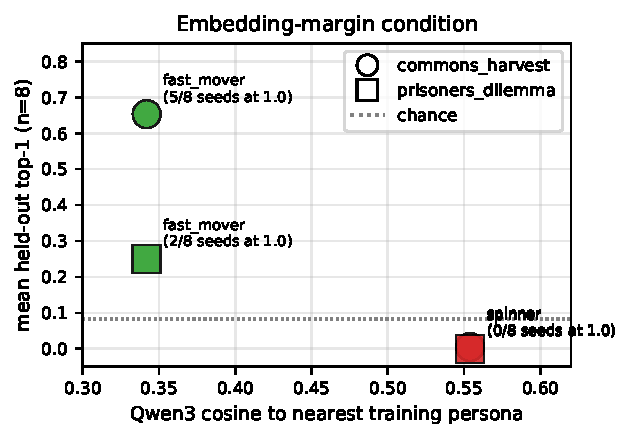
\includegraphics[width=0.65\linewidth]{fig3_embedding_margin.pdf}
  \caption{Per-persona mean held-out top-1 ($n=8$) plotted against cosine
  distance to the nearest training persona. The crowded held-out persona
  (\texttt{spinner}, cosine $0.554$) is unrecoverable on both substrates;
  the well-isolated persona (\texttt{fast\_mover}, cosine $0.342$) is
  recoverable on a substantial fraction of seeds.}
  \label{fig:margin}
\end{figure} The \PCSP projection head, under any seed
of the persona-balanced \InfoNCE configuration we have tested, cannot place a
decision boundary in regions denser than the corpus's maximum pairwise
cosine. This is a falsifiable per-persona predictor of recovery and the
mechanistic content of the H3 result.

% --------------------------------------------------------------------
\section{Discussion}
\label{sec:discussion}

The H3 configuration that recovers held-out personas pays a cost: in-
distribution top-3 retrieval on the same configuration drops to chance
($0.225\,[0.181,\,0.281]$ vs.\ $0.250$). The same projection geometry that
admits held-out personas abandons in-distribution discriminability over the
$10$ training personas. We read this as a constraint on the single-objective
\InfoNCE formulation: the projection head can either separate $10$ training
personas or admit $2$ held-out personas, but not both at the configuration
class we have tested. A multi-objective formulation that adds a per-cluster
pinning term to retain in-distribution structure while still admitting held-
out recovery is the natural next step but is out of scope for this paper.

Cross-cutting these results is the bimodality finding: the \InfoNCE
projection head is a discrete two-attractor optimization landscape whose
basin of attraction is determined by initial conditions of the projection
parameters and not by reward dynamics. Wrapping a re-seeding strategy around
the projection-head training is in principle tractable; doing so would convert
the conditional H3 result into a deterministic one.

% --------------------------------------------------------------------
\section{Limitations}
\label{sec:limits}

The persona corpus is small ($12$ personas); the embedding-margin condition
is therefore exposed by a single held-out persona's geometry rather than by a
controlled-margin sweep. Three substrates from distinct categories establish
H1 robustly but do not exhaust the Melting Pot benchmark. We did not test
H4 (persona-edit controllability) or H2 (convention emergence) in this
paper; a pre-registered H4 protocol is committed but not yet executed. A
preliminary $\lambda_{\text{IC}}$ sweep on \cH and \stag returned a
degenerate Pareto frontier between identification and reward, which we
interpret as evidence that the bottleneck is the projection-head landing
condition rather than a continuous identity--reward trade-off; a fuller H5
study at smaller $\lambda$ steps and across more substrates is the natural
extension.

% --------------------------------------------------------------------
\section{Conclusion}
\label{sec:conc}

Persona-conditioned shared policies produce distinguishable behavior under
multi-agent strategic pressure on three Melting Pot substrates with
bootstrap-separated CIs (H1). On \cH, persona-balanced \InfoNCE training
recovers held-out personas at top-3 accuracy bounded away from chance
($0.480\,[0.257,\,0.696]$, $n=8$, H3). The recovery is governed jointly by an
embedding-geometry condition (held-out personas must not be crowded against
training personas) and by a discrete projection-head basin-landing condition;
neither is visible without multi-seed evaluation. The bimodality is a
phenomenon of the \InfoNCE projection head, not of PPO. Both the
embedding-margin condition and the basin-landing dynamics suggest concrete
mechanistic targets (controlled-margin held-out corpora; multi-objective
\InfoNCE with per-cluster pinning) for converting the conditional H3
recovery into a deterministic one.

% --------------------------------------------------------------------
\bibliographystyle{plain}
\bibliography{refs}

% --------------------------------------------------------------------
\appendix

\section{Hyperparameters}
\label{app:hparams}

PPO: $8$ vectorized environments, $128$-step rollouts, $4$ minibatches, $4$
update epochs per rollout, learning rate $2.5 \times 10^{-4}$, entropy
coefficient $0.01$, total budget $1\,000\,000$ environment steps per run.
\InfoNCE: trajectory-encoder hidden size $128$, output dimension $64$,
temperature $0.1$, $\lambda_{\text{IC}} = 0.5$, $\lambda_{\text{KL}} = 0$.
Persona conditioning: concat with $1024$-dimensional frozen Qwen3 embedding.
Diagnostics every $25$ updates; checkpoints every $200$ updates.

\section{PD held-out recovery details}
\label{app:pd}

\PD held-out retrieval, $n=8$ seeds, persona-balanced \InfoNCE
configuration: \textsc{heldout/random} full top-1 $0.109\,[0.000,\,0.273]$,
full top-3 $0.297\,[0.078,\,0.539]$, heldout\_only top-1
$0.469\,[0.438,\,0.500]$. Positive-basin landing rate $2/8$. The smaller
per-update batch on \PD ($2$-player substrate, $16$ trajectories per update
vs.\ \cH's $7$-player $56$) reduces the persona-balanced batch's per-step
diversity and is the mechanically consistent reason for the lower landing
rate.

\section{PPO stability across basins}
\label{app:ppo}

Episode return mean, value-function loss, and approx-KL trajectories of
positive-basin and zero-basin seeds on \cH are visually indistinguishable
through the entire $1$~M-step training budget. No training divergence,
value-function collapse, or entropy collapse was observed in any of the
$16$ seed--substrate combinations contributing to Sections \ref{sec:h3} and
\ref{sec:bimodality}. The two basins differ at the projection-head
trajectory embedding $z_\tau$ at convergence; the policy network and value
function do not.

\end{document}
